%\section{Spiking Neural Networks}
\label{sec:application:snn}

%describe alternatives for the spike response and refractoriness functions

This section explains how we have implemented a spiking neural network and the results obtained after using it with the signals of our scenario. 

We emphasize that the MatLab Toolbox for neural networks does not have any library for SNN. We searched and tried to use third-party software, but they were not enough suitable for our experiment. Therefore, we opted for implementing the entire code in MatLab.






\subsection{Codification}
\label{subsec:codification}
The main characteristic of a SNN is that its inputs and outputs are not the signal values, but the time references of the spiking train of its neurons. Hence, the first step we must carry out is to encode continuous input variables in spike times.

There are three different ways of performing this codification process \cite{stromatias2011developing}:
\begin{itemize}
\item Rate coding, in which the	information	is encoded into	the	mean firing rate of the neuron iduring a time window.
\item Temporal coding, in which the form of spike times encodes the information.
\item Population coding, in wich the representation of analog input variables is encoded by a population of neurons whose firing times are determined by the value of the signal.
\end{itemize}

We chose for our experiment the latter codification because it is the most suitable when dealing with a low number of input signals and it is a well studied method for representing real-valued parameters. 
More precisely, we employed an encoding based on arrays of Gaussian Receptive Fields (GRF) which associate highly stimulated neurons with early firing times and less stimulated neurons with later (or no) firing times.

In our encoding process, the number of GRF used was set to $m=3$. Firstly, the input data is normalized between the values $I_{\text{max}}$ and $I_{\text{min}}$. Then, the gaussian parameters of each GRF are calculated as follows:
\begin{equation}
C_{i}=I_{\text{min}}+\frac{2i-3}{2}\frac{I_{\text{max}}-I_{\text{min}}}{m-2}
\end{equation}
\begin{equation}
\sigma_{i}=\frac{1}{\gamma}\frac{I_{\text{max}}-I_{\text{min}}}{m-2}
\end{equation}
where $C_{i}$ and $\sigma_{i}$ are the center or mean and the standard deviation of the $i$-th gaussian of the $m$ GRFs. $\gamma$ is a constant number usually around $1.5$. A threshold has to be used so that GRF neurons below that critical value should not fire.
\figref{grfencoding} shows an example in which a normalized heart rate sample is encoded into firing times with a threshold of $0.15$ and a maximum delay of spike of $20$.

\begin{figure}[!ht]
\centering
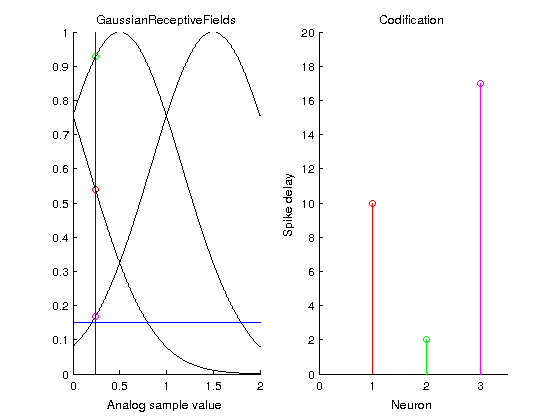
\includegraphics[width=0.9\columnwidth]{images/results/encondingINnorm.png}
\caption{Population coding with Gaussian Receptive Fields}
\label{fig:grfencoding}
\end{figure}





\subsection{Implementation of the Spike Response Model}
\label{subsec:srmimplementation}
The first step for implementing the SRM of spiking neurons described in \subsubsecref{SRM}, is to select the refractory $\eta$ and spike response $\varepsilon$ functions. 

Beginning with the spike response function, it has to model the sudden increase of the membrane voltage. Among the curves that suit the membrane potential curve, we chose the following, which is described in \cite{booij2004temporal}:
\begin{equation}
\varepsilon(s)=\frac{s}{\tau}\text{exp}(1-\frac{s}{\tau})\mathcal{H}(s)
\label{eq:spikeresponsefunction}
\end{equation}
where $\tau$ is a time constant set to $2.7$ that controls the rise- and decay-time and $\mathcal{H}(s)$ denotes the Heavy-side step function:
\begin{equation}
\mathcal{H}(s)=
	\begin{cases}
    	0 & \text{if } s \leq 0\\
    	1 & \text{if } s > 0
  	\end{cases}
  	\label{eq:heaviside}
\end{equation}
which makes $\varepsilon(t)$ accomplish the condition of $\varepsilon(t)=0~\text{for}~t\leq 0$. \figref{spikeresponsefunctionPlot} depicts the spike response function we used.
\begin{figure}[!ht]
\centering
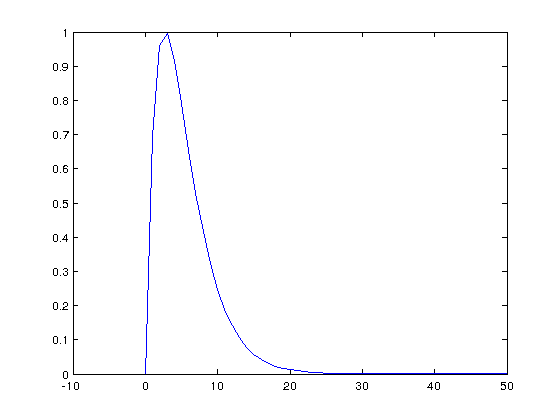
\includegraphics[width=0.82\columnwidth]{images/results/spikeresponsefunction.png}
\caption{Spike response function}
\label{fig:spikeresponsefunctionPlot}
\end{figure}

Then, the refractory function has to model the negative overshoot of the action potential. Again, among the possible implementations we chose the one exposes in 
\cite{booij2004temporal}:
\begin{equation}
\eta(s)=-\vartheta \text{exp}(-\frac{s}{\tau_{r}})\mathcal{H}(s)
\label{eq:refractoryfunction}
\end{equation}
where $\vartheta$ is the threshold of the neuron, $\tau_{r}$ is a another time constant set to $20$ and $\mathcal{H}(s)$ the Heaviside function of \eref{heaviside}, which make the refractory function accomplish the condition $\eta(t)=0~\text{for}~t\leq 0$. \figref{refractoryfunctionPlot} depicts the refractory function we used.
\begin{figure}[!ht]
\centering
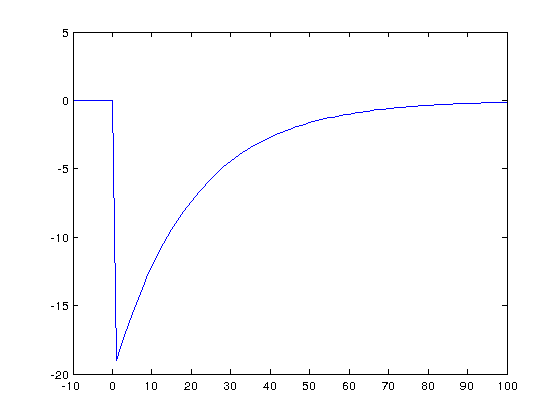
\includegraphics[width=0.82\columnwidth]{images/results/refractoryfunction.png}
\caption{Refractory function}
\label{fig:refractoryfunctionPlot}
\end{figure}



\subsection{Implementation of the Spiking Neural Network}
\label{subsec:snnimplementation}
The SNN we have implemented tries to solve the same scenario as the other ANNs analysed; \ie, its parameters are set in in a manner that the resultant SNN can be compared with the other models in terms of prediction horizon (30 minutes). Other parameters related to the topology are not comparable because of the differences in the type of ANNs.

Hence, our SNN has, for each physiological signal, a number of input neurons equal to the amount of GRFs used for encoding the analog values. Therefore, in our net there are 3 neurons for each signal source, which means a total of 12 neurons in the input layer. All these neurons are connected to the output layer, which has a unique neuron.

We configured the network in order to have $m=2$ synapses in each connection between input-neurons and output-neuron. Then, the $k$-th synapse has a delay of $d_{k}=k$ units of time.

For dealing with the maximum delay encoded with the GRFs (see \subsecref{codification}) we windowed all signals. We set the window length equal to this maximum delay (20 units of time) and combined the spikes that fired within the window removing the repeated delays. This way, if an analog value was encoded with delays $d_{GRF_{1}}=8$ and $d_{GRF_{2}}=2$ and, within the same window, another analog value was encoded with $d_{GRF_{1}}=8,d_{GRF_{2}}=5$ and $d_{GRF_{3}}=16$, then, the final spike train that encodes the entire window is $d_{GRF_{1}}=8, d_{GRF_{2}}=[2,5]$ and $d_{GRF_{1}}=16$. 

We implemented every equation of the spike backpropagation algorithm in MatLab. Every step, the signal window is shifted without overlapping, \ie, it is shifted a number of units of time equals to the window length. 
\begin{figure}[!ht]
\centering
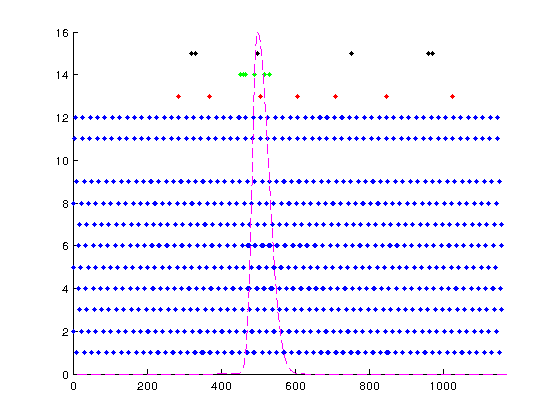
\includegraphics[width=0.85\columnwidth]{images/results/snn1.png}
\caption{Graphic example of the SNN application}
\label{fig:snnResults}
\end{figure}

\figref{snnResults} shows a grahical example we obtained. In the plot, the y-axis and x-axis represent each neuron and the time respectively. Thus, a point in $x=57, y=4$ depicts a spike in $t=57$ of the $4^{\text{th}}$ neuron. The red points correspond to the original output spikes; the green ones, to the encoded target signal and black ones to the output spikes after training the network. The blue points are the spikes of the input neurons, so that neurons 1-3 fire because of the HR signal, 4-6 because of the EDA variable, 7-9 corresponds to TEMP signal and the Sp02 is encoded in neurons 10-12. The pink curve represents the analog target signal just for a better visualization of the important timestamps. A zoomed plot can be observed in \figref{snnResultsZoom} in order to indicate that spikes are not as periodically as they seem.
\begin{figure}[!ht]
\centering
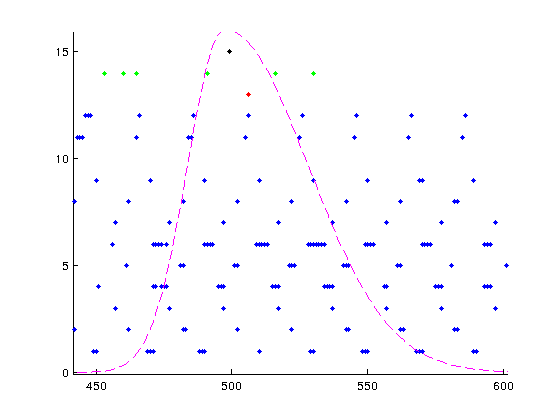
\includegraphics[width=0.85\columnwidth]{images/results/snn1zoomed.png}
\caption{Zoomed plot of spikes distribution}
\label{fig:snnResultsZoom}
\end{figure}

Notice that physiological signals were encoded into three spikes-train, one for each GRF used. However, we have a single output neuron and therefore we must encode the target signal into a unique sequence of spikes. We carried out this process by applying a little SNN: 
\begin{enumerate}
\item The analog target curve is firstly encoded the same way as physiological signals (3 GRFs).
\item A SNN of three-neurons input and one-neuron output layers is build. Each connection with the same number of synapses as the principal SNN ($m=2$) and a delay of $d_{k}=k$ for the $k$-th synapse too.
\item The encoded analog target signal is presented to the just build SNN, so that the output of the net comprises the codification of the target signal for the principal SNN.
\end{enumerate}

Following this process, we can observe how the output neuron begins to fire (green points in \figref{snnResults}) before the analog target signal arrives to the pain gaussian (pink curve in \figref{snnResults}). 
The first firing time of this spike traine fixes our prediction horizon. 
Also the output neuron stops firing after the target signal decrease its value, which indicate that the reset process can be carried out successfully.

Unfortunately, our implementation of the backpropagation algorithm does not make the SNN learn correctly: 
the output neuron spikes too many times. 
Consequently, the SNN developed cannot be used as predictor because of the multiple false positives it would produce. 
Besides, the NARX model generates a greater forecasting horizon, concluding that one can perform better predictions.
